
\chapter{Come funziona il sistema Bitcoin?}
\label{chap:basi}

\vspace*{1cm}

\section{Crittografia}
\subsection{Introduzione}
\label{sec:sezioni}
Molte delle propriet\`a dei Bitcoin sono possibili grazie alla crittografia, con la quale possono essere generate chiavi digitali, indirizzi Bitcoin e firme digitali.
Bitcoin fa uso di una crittografia \textit{asimmetrica o a chiave pubblica}.
In questo tipo di crittografia ogni utente possiede una coppia di chiavi, una chiave privata e una chiave pubblica, utilizzate per criptare e decriptare delle informazioni che gli stessi si scambiano in un messaggio. Questo tipo di crittografia risulta molto pi\`u efficace rispetto alla crittografia simmetrica, in cui i corrispondenti cifrano e decifrano i dati scambiati utilizzando un'unica chiave segreta (ma in questo caso sorge il problema
di come scambiarsi in maniera sicura la chiave stessa).
La chiave privata \`e, appunto, tenuta segreta dal suo possessore, mentre chiave la pubblica pu\`o essere resa nota. La chiave pubblica \`e generata a partire dalla privata attraverso una funzione non iniettiva, ovvero dalla chiave pubblica \`e impossibile risalire alla chiave privata da cui deriva. Infine chiave privata e chiave pubblica hanno una specifica e diversa funzione: la chiave pubblica serve cifrare le informazioni da
inviare, informazioni che possono essere decifrate soltanto con la relativa chiave privata. 
Bitcoin si basa su una particolare crittografia asimmetrica chiamata \textit{moltiplicazione su curva ellittica} che offre un meccanismo per la creazione di una coppia di chiavi, una chiave pubblica che \`e usata per ricevere denaro, e una chiave privata usata invece per firmare le transazioni e spendere fondi.
La \textbf{chiave privata (k)} \`e semplicemente un numero casuale, poi da questa chiave usando appunto l' \textit{elliptic curve multiplication} si genera la chiave pubblica, dalla quale infine facendo uso di una \textit{funzione di hash} \footnote{Una funzione di hash h, \`e una funzione che mappa un messaggio arbitrariamente lungo in una stringa di lunghezza prefissata, cercando di far in modo che da questa stringa non si possa risalire al messaggio che l'ha generata.} \`e possibile generare l'\textit{address} (indirizzo Bitcoin) dello user.\\
Per creare la chiave privata si prendono 256 bit in modo casuale e si controlla che il numero risultante sia minore di un certo valore \textit{n} \footnote{In Bitcoin n=1,${1,158\times 10}^{77}$.} , in caso negativo si ripete l'esperimento rigenerando un altro numero casuale nello stesso modo.\\
La \textbf{chiave pubblica (K)} \`e calcolata dalla privata (k) usando la moltiplicazione su curva ellittica:
\begin{equation}
K=k\times G
\end{equation}
ove G \`e la costante di generazione di punti sulla curva. 

 
\subsection{Crittografia su curva ellittica}
\label{sec:sezioni}
La crittografia usata da Bitcoin si basa una particolare curva ellittica chiamata \textit{secp256k1} , definita dalla funzione:
\begin{equation}
{y}^{2} \mod p= ({x}^{3} +7) \mod p
\end{equation}\\
Notiamo che ci troviamo in un caso discreto, la curva sar\`a quindi descritta da solamente alcuni punti sugli assi cartesiani.\\
(Per semplificare il ragionamento possiamo pensare al caso reale, \textit{figura 2.1})
\begin{figure}[!hb]
   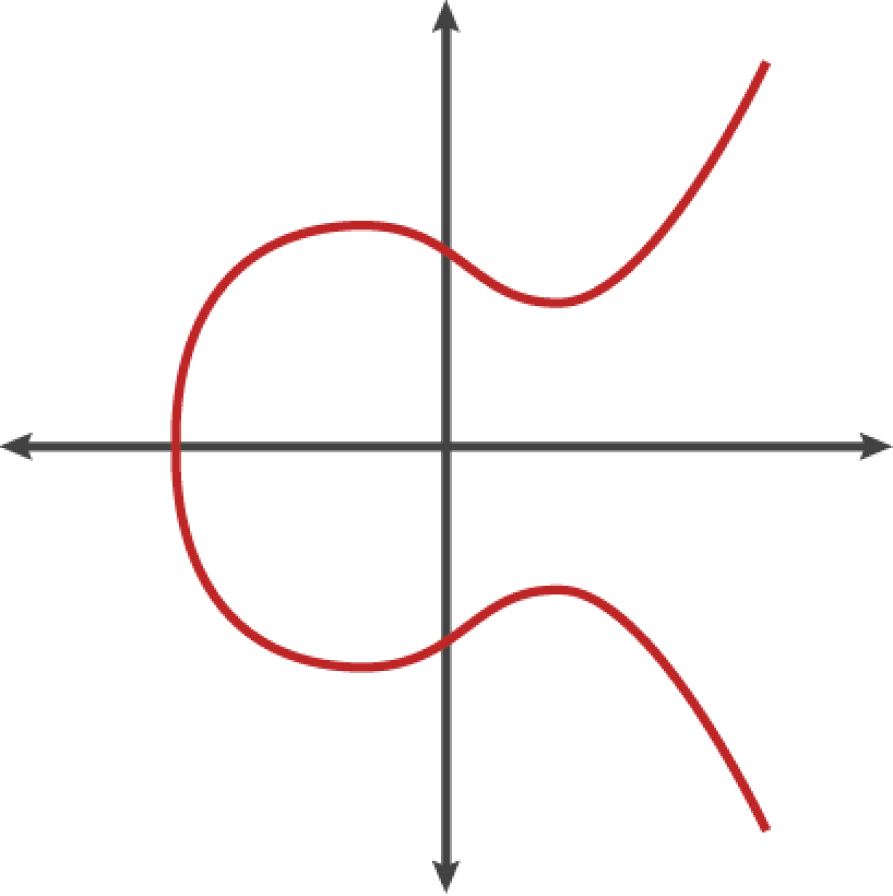
\includegraphics[width=0.375\textwidth]{imgs/mbc2_0402.png}
   \hfill
   \caption{Crittografia su curva ellittica: visualizzazione della curva ellittica con p=17, caso continuo}
   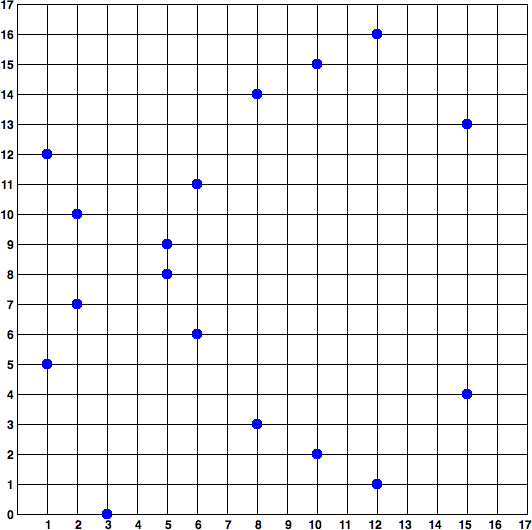
\includegraphics[width=0.375\textwidth]{imgs/mbc2_0403.png}
   \caption{Crittografia su curva ellittica: visualizzazione della curva ellittica con p=17, caso discreto}
\end{figure}\\Una propriet\`a fondamentale di questa curva \`e che dati due punti $P_1$ e $P_2$ $\in $ ad essa, allora anche $P_3=P_1+P_2 \ \in $ alla curva. 
Possiamo pensare alla moltiplicazione tra due punti della curva nel seguente modo:
se voglio moltiplicare un punto per un dato numero K, baster\`a sommare il punto a se stesso K volte, in questo modo risulta molto semplice ricavare la \textit{public key} dalla \textit{private key} attraverso la \textit{2.1.1}\\


\subsection{Indirizzi Bitcoin}
\label{sec:sezioni}
Un indirizzo Bitcoin  viene prodotto da una chiave pubblica, e consiste in una stringa che inizia con "1". Un indirizzo  pu\`o rappresentare il possessore di una coppia di chiavi (\textit{public/private key}) oppure qualcos'altro come uno script di pagamento.\\
Partendo dalla chiave pubblica ,vengono applicate due funzioni di hash,  uno \textit{SHA256} e poi \textit{RIPEMD160} sul risultato, ottenendo un numero a 160 bit (20 byte) che rappresenter\`a l' \textit{address} dell'utente:\\\\
$ A_{address}=RIPEMD160(SHA256(K))$\\\\
Gli indirizzi Bitcoin sono codificati in \textit{Base58Check} per proteggersi dagli errori umani. Questo formato \`e utilizzato perch\`e elimina i caratteri tra loro fraintendibili per l'occhio umano, inoltre sempre per prevenire un errore che pu\`o venire commesso da un utente la codifica \textit{Base58Check} crea un meccanismo di \textit{check} (controllo). Il \textit{checksum} \footnote{In telecomunicazioni e informatica il checksum  \`e una sequenza di bit che viene utilizzata per verificare l'integrit\`a di un dato o di un messaggio che pu\`o subire alterazioni durante la trasmissione sul canale di comunicazione.} sono 4 byte che vengono aggiunti alla fine dell'indirizzo, e derivano dalla funzione \textit{hash} di tutto quello che li precede, cosi possiamo sempre controllare la correttezza di un indirizzo.\\
Per convertire dei numeri (dati) in \textit{Base58Check} , per prima cosa creiamo un prefisso chiamato \textit{version-byte} che indica il tipo di dato, ad esempio per un indirizzo Bitcoin \`e 0 ( 0x00 in hex).\\
Poi si crea un checksum con un \textit{double SHA}:\\\\
$checksum=SHA256(SHA256(prefix+data))$\\\\
Dai 32 byte che risulteranno da questo procedimento prendo solo i primi 4.\\
Il risultato finale \`e quindi composto da: \textit{prefix,data,checksum}.
Il prefisso cambier\`a a seconda di cosa voglio codificare.
\begin{figure}[!h]
   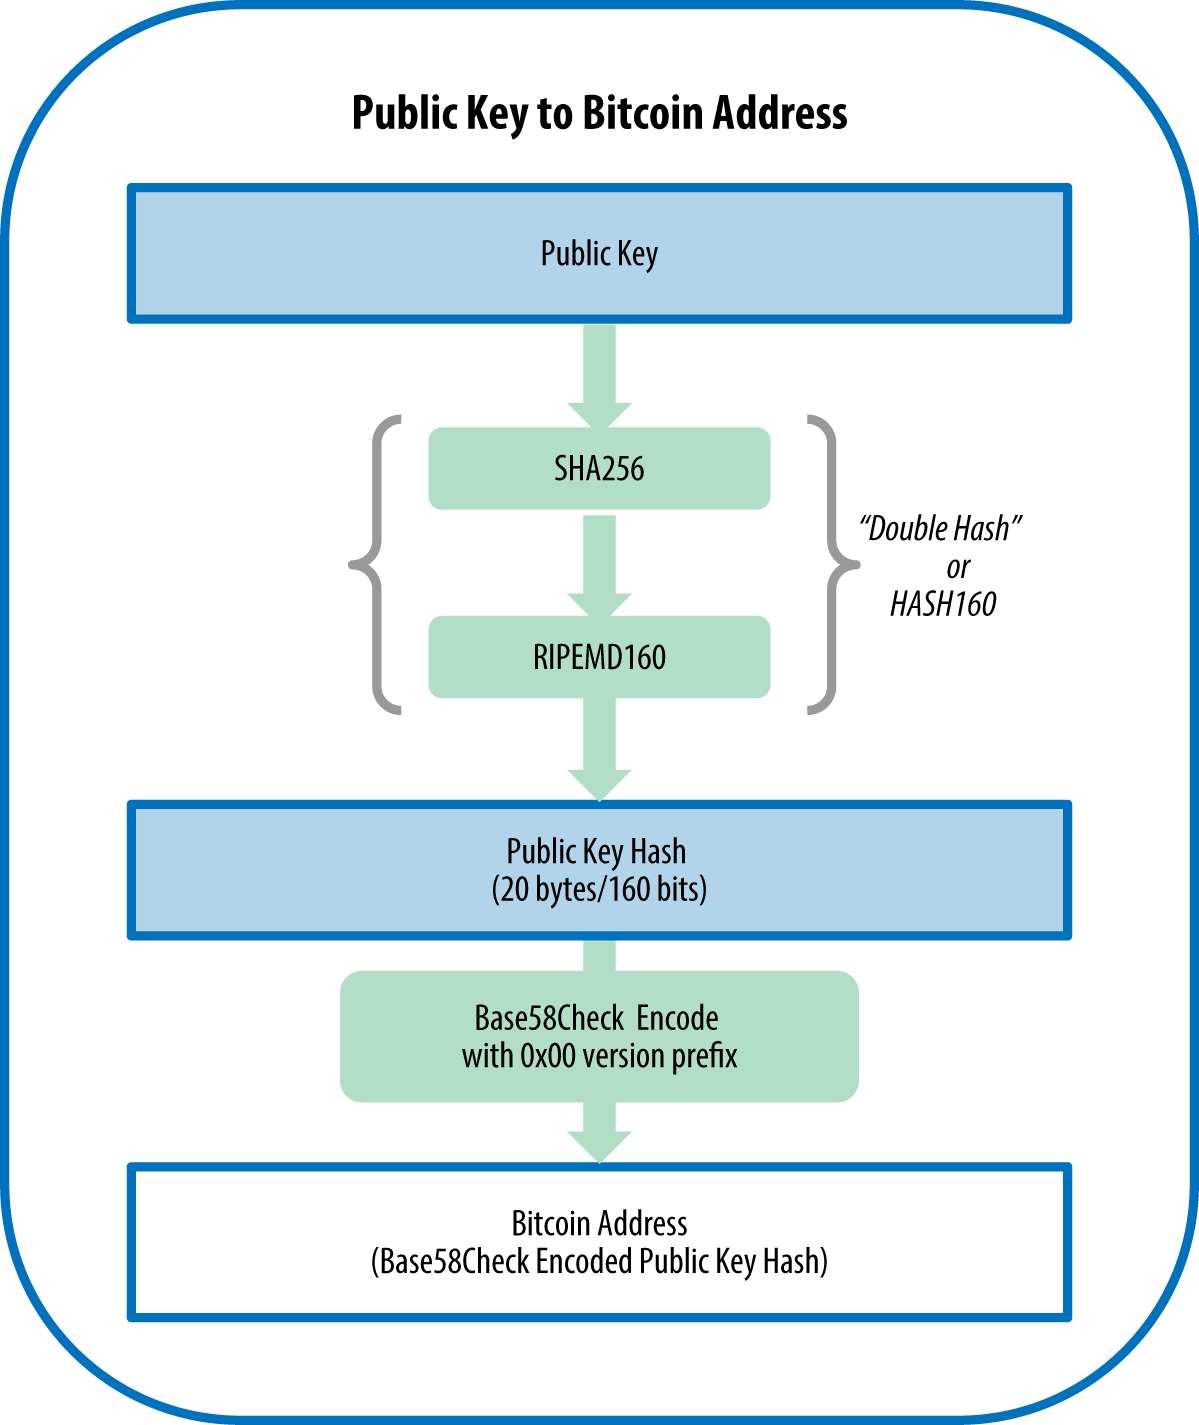
\includegraphics[width=0.675\textwidth]{imgs/address.png}
   \caption{Conversione da una chiave pubblica ad un indirizzo Bitcoin}
\end{figure}



\section{Le transazioni}
Le transazioni sono delle strutture dati che codificano il trasferimento di valori tra partecipanti del sistema Bitcoin, forniscono quindi agli utenti la possibilit\`a di spendere satoshis \textit{una sottounit\`a di bitcoin, che pu\`o essere paragonata ai centesimi di Euro}. Ogni transazione \`e composta da diversi elementi, che danno la possibilit\`a di poter svolgere a parimenti transazioni semplici e pi\`u complesse, a seconda delle esigenze.
Ogni nodo nel network Bitcoin dovrebbe essere in grado di trasmettere le transazioni nel network e farle minare in un blocco. 
Inoltre, ogni nodo dovrebbe essere in grado di controllare se:
\begin{itemize}
\item Il denaro speso nella transazione esiste realmente.
\item Il denaro \`e gi\`a stato utilizzato (problema del \textit{double spending}).
\item Chi spende il denaro ha effettivamente i diritti per poterlo fare.
\end{itemize}
L'idea generale delle transazioni nel network Bitcoin \`e quella di inviare degli Input che vanno a spendere degli Output. Ogni transazione ha quindi almeno un Input ed un Output. Ogni Input spende un Output precedente.
Ogni Output \`e quindi in una specie di sala d'attesa (e prende il nome di Output Non Speso, \textit{\textbf{UTXO}}), finch\`e un successivo Input non lo "spende".
Ogni transazione ha come prefisso il numero della versione, che ha lo scopo di indicare agli altri \textit{peer} ed ai \textit{miner} il corretto insieme di regole da usare per validarla. Questo da la possibilit\`a agli sviluppatori di poter creare nuove regole senza invalidare le transazioni precedenti.

\subsection{UTXO: output di transazione non spesi}
Gli output nelle transazioni sono pezzi indivisibili di bitcoin registrati nella \textit{blockchain}. Un \textit{full node} della rete traccia tutti gli output spendibili, conosciuti come \textbf{\textit{unspent transaction outputs UTXO}}. Ogni transazione rappresenta un cambiamento nell'insieme di UTXO. Quindi quando diciamo che il \textit{wallet} di uno user ha "ricevuto" bitcoin, intendiamo dire che il \textit{wallet} ha trovato un UTXO che pu\`o essere speso usando le proprie chiavi. Lo \textit{ user's bitcoin balance} \`e la somma degli UTXO che lo user pu\`o spendere.\\
Come un centesimo non pu\`o essere suddiviso, un Bitcoin non pu\`o essere suddiviso sotto l'ottavo decimale del \textit{satoshis}. Sebbene un output pu\`o avere un valore qualunque, una volta creato questo \`e indivisibile, gli output sono appunto \textbf{discreti} e \textbf{indivisibili}.
Ad esempio, se si possiede uno UTXO di 20 bitcoin e si vuole pagare 1 bitcoin, la transazione generata deve consumare tutti e 20 i bitcoin producendo 2 output, 1 BTC all'address desiderato, e gli altri 19 BTC al tuo proprio \textit{wallet} (come se fosse il resto).\\L'applicazione \textit{wallet} di uno user tipicamente seleziona tutti gli UTXO dello stesso per arrivare alla quantit\`a desiderata, per poter cosi effettuare il pagamento.\\C'\`e per\`o un'eccezione a questa catena di input e output, una speciale transazione chiamata \textbf{coinbase transaction}, che \`e la prima transazione contenuta in ogni blocco della blockchain. Questa transazione \`e posta li dal miner "vincente" e crea dei bitcoin spendibili dal miner stesso. La \textit{ coinbase transaction} non consuma UTXO, invece ha un input speciale chiamato \textit{coinbase}. Questo \`e come i Bitcoin vengono creati durante il processo di \textit{mining}.

\subsection{I fees di transazione}
La maggior parte delle transazioni includono \textit{fees}, delle ricompense in bitcoin per il lavoro svolto dai \textit{miner}. Analizziamo pi\`u in dettaglio come i fees vengono inclusi nelle transazioni. La maggior parte dei \textit{wallet} calcola e include \textit{fees} automaticamente.\\
Le \textit{transaction fees} (fees di transazione) servono come incentivo per includere (minare) una transazione nel prossimo blocco, possiamo vederle come una sorta di commissione.\\
Le \textit{transaction fees} sono calcolate in base alla dimensione della transazione in kilobytes, non in base al valore in BTC di essa, come si potrebbe pensare. I miner danno priorit\`a alle transazioni da includere nel blocco che sono in procinto di minare in base a vari criteri, tra questi c'\`e proprio la quantit\`a di 	\textit{fees} che ricaverebbero includendo una data transazione in tale blocco. Una transazione con sufficienti \textit{fees} \`e perci\`o pi\`u favorevole ad essere inclusa nel prossimo blocco, se invece i \textit{fees} sono troppo pochi la transazione pu\`o essere ritardata o addirittura neanche processata. Una transazione con \textit{fees} possimi allo zero rischia di non essere neanche propagata nel network.\\
Nel \textit{Bitcoin Core} (implementazione di riferimento di bitcoin) la politica dei \textit{fees} \`e settata dal \textbf{\textit{minerlayfee option}}. Attualmente il \textit{minerlayfee} \`e 0.00001 BTC per kilobyte.\\
Un algoritmo chiamato \textit{Fees Estimation Algorithm} calcola un ammontare di \textit{fees} appropriato affinch\`e i \textit{fees} offerti rendano la transazione competitiva all'interno del network. Si stima tramite questo algoritmo la quantit\`a necessaria di \textit{fees} che dia alla transazione un' alta probabilit\`a di essere inclusa da qui ad un certo numero di blocchi a venire. I servizi offrono di solito una alta, media, bassa probabilit\`a a seconda di della quantit\`a di \textit{fees} che si \`e disposti a pagare.\\


\subsection{Linguaggio di script delle transazioni}
L'\textit{engine} di validazione delle transazioni Bitcoin si basa su due tipologie di script, \textit{locking script} e \textit{unlocking script}.\\
Il \textit{locking script}  \`e posto su un output: specifica la condizione da soddisfare affinch\`e si possa spendere questo output in futuro. Il \textit{locking script} \`e chiamato anche \textit{scriptPubKey, witness script o cryptographic puzzle}.\\
L' \textit{unlocking script} risolve le condizioni poste su un output attraverso il \textit{locking script}, questa \`e parte dell'input di ogni transazione. Molto spesso gli \textit{unlocking script} contengono la firma digitale del \textit{wallet} dello user, prodotta dalla sua chiave privata.\\
L'algoritmo di firma digitale usato nei Bitcoin \`e l' \textit{Elliptic curve digital signature algorithm ECDSA}. La firma digitale ha tre scopi in Bitcoin:
\begin{enumerate}
\item La firma digitale d\`a prova della propriet\`a di una chiave privata, cio\`e del possessore dei fondi.
\item La prova dell' autorizzazione (a spendere) \`e innegabile.
\item La firma prova che la transazione non pu\`o e non deve essere modificata da nessuno dopo che \`e stata firmata.
\end{enumerate}
Ogni nodo di validazione dei Bitcoin, valider\`a le transazioni eseguendo il \textit{locking} e l' \textit{unlocking} script insieme. Il software di validazione copier\`a l' \textit{unlocking script}, prender\`a l' \textit{UTXO} referenziato dall'input, e copier\`a il  \textit{locking script} di questo \textit{UTXO}. Ora i due script saranno eseguiti in sequenza. Ci sar\`a la convalida se l' \textit{unlocking script } soddisfer\`a le condizioni del \textit{locking script}. Tutti gli input sono convalidati indipendentemente.
Il linguaggio di script della transazione Bitcoin \`e chiamato \textbf{Script}.
Questo contiene molti operatori, ma non contiene loop, solamente controlli condizionali. Il linguaggio quindi \textbf{\textit{non \`e Turing completo}}. Queste limitazioni permettono di non creare loop infiniti che possono essere usati come \textit{denial of service attack} contro la rete Bitcoin (Ricorda ogni transazione \`e validata da ogni full node).

\section{La rete Bitcoin }

\subsection{Architettura di rete peer-to-peer}
Il sistema Bitcoin \`e strutturato su un' architettura di rete \textit{peer-to-peer (\textbf{P2P})}. Con questo termine si indica che i computer che fanno parte della rete sono appunto "alla pari", non ci sono nodi "speciali", e perci\`o ogni nodo si assume la responsabilit\`a del funzionamento dei vari servizi di rete. Non c'\`e un server, non ci sono servizi centralizzati, e alcun tipo di gerarchia all' interno della rete. I nodi nella rete \textit{P2P} forniscono e allo stesso tempo consumano i servizi offerti dalla stessa. La caratteristica principale quindi di tale rete \`e il fatto di essere decentralizzata e aperta a chiunque. All'infuori di Bitcoin le applicazioni che hanno avuto pi\`u successo su questa architettura di rete sono \textit{Napster} e  \textit{BitTorrent}.\\
Bitcoin \`e nato per essere un sistema di moneta digitale su rete \textit{P2P}, e la decentralizzazione del controllo \`e il cuore dei principi di Bitcoin, e questa pu\`o essere raggiunta solamente sfruttando le caratteristiche di una tale rete.\\
Il termine \textit{Bitcoin Network} si riferisce all' insieme di nodi che stanno eseguendo il protocollo \textit{Bitcoin P2P}.

\subsection{I ruoli dei partecipanti della rete Bitcoin}
Sebbene i nodi in una rete \textit{P2P} siano alla pari, questi possono avere compiti differenti all'interno di essa. Un nodo Bitcoin implementa 4 diverse funzionalit\`a fondamentali:
\begin{itemize}
\item routing 
\item blockchain database
\item mining
\item servizi wallet
\end{itemize}
\begin{figure}[htb]
\begin{center}
   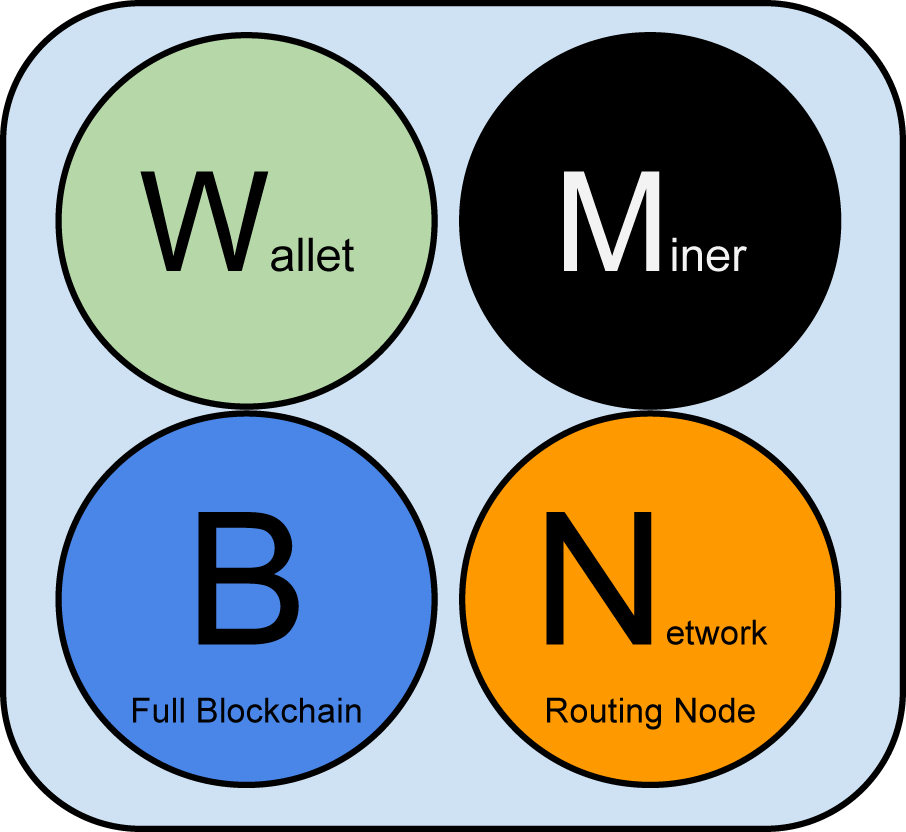
\includegraphics[width=0.355\textwidth]{imgs/4Funzioni.png}
   \caption{Un nodo della rete Bitcoin con tutte e quattro le funzionalit\`a: \textit{wallet, miner, full blockchain database e network routing}}
   \end{center}
   \hfill
\end{figure}
Tutti i nodi includono la funzioni di \textit{routing} per partecipare alla rete. Ogni nodo valida e propaga le transazioni e i blocchi sulla rete, inoltre scopre e mantiene connessioni verso altri \textit{peer}.\\
Alcuni nodi, chiamati \textit{full nodes}, mantengono anche una copia aggiornata della \textit{blockchain}. I \textit{full nodes} posso quindi verificare in autonomia le transazioni senza aver bisogno di referenze esterne. Alcuni nodi mantengono invece solamente una parte di tutta la \textit{blockchain}, e verificano le transazioni usando un metodo chiamato \textit{simplified payement verification , SPV}. Questi nodi sono chiamati nodi SPV o nodi \textit{lightweight}.\\
I nodi \textit{miner} competono per creare nuovi blocchi, utilizzando hardware dedicato alla risoluzione dell' algoritmo di \textit{Proof-of-work}. Alcuni nodi \textit{miner} sono anche \textit{full node}, cio\`e hanno una copia dell' intera \textit{blockchain}, mentre altri sono nodi \textit{lightweight} che partecipano a \textit{pool} di \textit{mining} dove soltanto il \textit{pool server} ha la funzionalit\`a di \textit{full node}.\\


\subsection{Come fa un nuovo partecipante a collegarsi alla rete Bitcoin?}
Quando un nuovo nodo si avvia, questo deve scoprire altri nodi all' interno della rete in modo da poter entrare a far parte dell'ecosistema Bitcoin. Per iniziare questo processo un nodo deve scoprire almeno un altro nodo all' interno della rete e connettersi con esso. La posizione geografica dei nodi \`e irrilevante, inoltre la topologia della rete Bitcoin non \`e geograficamente definita. Per questo, si pu\`o scegliere a caso qualsiasi nodo Bitcoin della rete.\\
Per connettersi a un \textit{peer} conosciuto, si stabilisce una connessione TCP, solitamente sulla porta 8333. Dopo aver stabilito la connessione, il nodo inizier\`a la fase di \textit{handshake} trasmettendo un messaggio denominato \textbf{\textit{version}} che contiene le seguenti informazioni:
\begin{itemize}
\item \textit{nVersion}:
La versione del protocollo Bitcoin P2P che il client "parla"
\item \textit{nLocalServices}:
Una lista di servizi locali supportati dal nodo
\item \textit{nTime}:
Il tempo corrente
\item \textit{addrYou}:
L'indirizzo IP del nodo remoto visualizzato da questo nodo
\item \textit{addrMe}:
L' indirizzo IP del nodo locale, come \`e stato scoperto dal nodo locale
\item \textit{subver}:
Mostra il tipo di software che sta girando su questo nodo
\item \textit{BestHeight}:
La lunghezza della blockchain 
\end{itemize}
Il messaggio di \textit{version} \`e sempre il primo messaggio inviato da ogni \textit{peer} agli altri \textit{peer}. Il \textit{peer} che riceve questo messaggio andr\`a a vedere se il nodo che sta provando a stabilire una connessione con lui \`e compatibile, facendo un check del campo \textit{nVersion}, in caso positivo risponder\`a con un messaggio di \textit{verack}.\\
\begin{figure}[!htb]
\begin{center}
   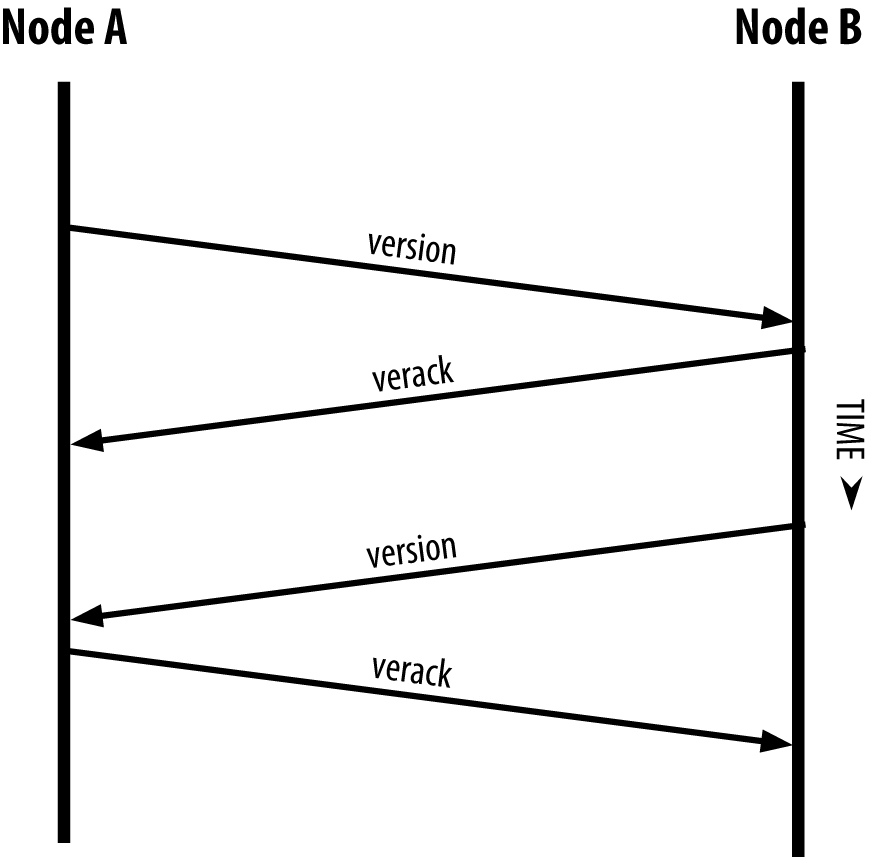
\includegraphics[width=0.455\textwidth]{imgs/connection.png}
   \caption{Handshake tra due peer della rete Bitcoin}
   \end{center}
   \hfill
\end{figure}\\\\
Come fa un nodo a trovare dei \textit{peer}?\\
Il primo metodo \`e facendo delle \textit{query DNS} a  dei \textit{DNS seeds} che sono server che forniscono indirizzi IP di nodi Bitcoin. Alcuni di questi \textit{DNS seeds} forniscono una lista statica di indirizzi di nodi Bitcoin stabili, altri invece ritornano un sottoinsieme random della lista degli indirizzi dei nodi Bitcoin collezionati da un \textit{crawler} della rete. Il \textit{Bitcoin Core} contiene al suo interno il nome di 5 differenti \textit{DNS seed}. Questi offrono un alto livello di affidabilit\`a per il processo iniziale di \textit{bootstrapping}.\\
Come alternativa, ad un nodo in fase di \textit{bootstrap} che non conosce nulla circa la rete, pu\`o essere fornito l' indirizzo IP di almeno un nodo che si trova nella rete, con il quale questo pu\`o stabilire una connessione e dal quale pu\`o ricevere maggiori informazioni riguardo la rete stessa. 
Una volta che una o pi\`u connessioni sono state stabilite, il nuovo nodo invier\`a un messaggio \textit{addr} ai suoi vicini contenente il proprio indirizzo IP. I vicini inoltreranno il messaggio \textit{addr} a loro volta ai loro vicini assicurandosi cos\`i che il nuovo nodo nodo sia ben connesso alla rete \footnote{Questo meccanismo di propagazione di messaggi all'interni di una rete viene chiamato \textit{gossip protocol}}. Il nuovo nodo in connessione pu\`o in aggiunta anche inviare un messaggio \textit{getaddr} ai suoi vicini, chiedendo loro di ritornare una lista di indirizzi IP di altri vicini.
\begin{figure}[!htb]
\begin{center}
   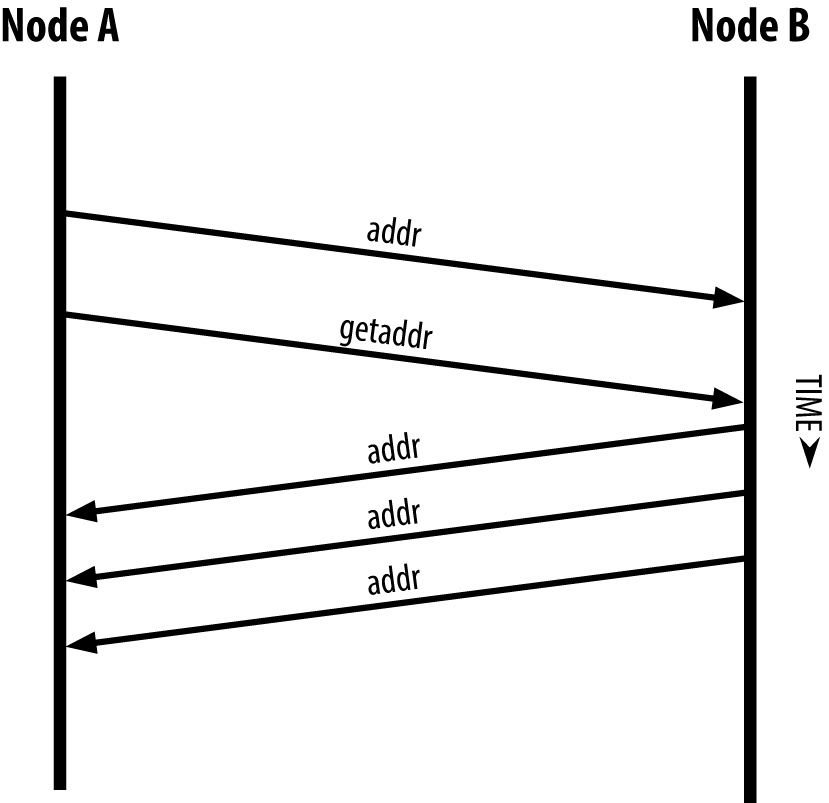
\includegraphics[width=0.455\textwidth]{imgs/addr.png}
   \caption{Propagazione di indirizzi Bitcoin}
   \end{center}
   \hfill
\end{figure}
Un nodo deve essere connesso ad alcuni \textit{peer} differenti in modo da poter stabilire dei path all' interno della rete Bitcoin. Questi path non sono del tutto affidabili, poich\`e i vicini di ogni nodo possono cambiare dinamicamente. Nella fase di \textit{bootstrap} c'\`e bisogno solamente di una connessione perch\`e questa fornir\`a informazioni su un altro nodo della rete che a sua volta far\`a in modo di collegarti a tutto il network. Dopo la fase di \textit{ bootstrap}, un nodo ricorder\`a un \textit{peer} con il quale \`e stato connesso, cos\`i ogni volta che verr\`a ravviato potr\`a collegarsi con questo senza passare nuovamente per la fase di \textit{bootstrap}.\\
Se non c'\`e traffico su una connessione, i nodi periodicamente si scambieranno dei messaggi per mantenere attiva la connessione, ma se questi smetteranno di comunicare per pi\`u di 90 minuti la connessione vierr\`a chiusa di default. Per questo la rete  \`e dinamica, pu\`o ingrandirsi o rimpicciolirsi senza un controllo centrale.

\subsection{Ricostruire la blockchain grazie al comando "Inventory"}
La prima cosa che deve fare un \textit{full node} che \`e appena entrato nella rete, \`e di provare a ricostruire tutta la \textit{blockchain}. Ogni nuovo nodo consce solo il primo blocco (\textit{genesis block} \footnote{Il genesis block pu\`o essere visualizzaro al link : https://www.blockchain.com/it/btc/block/000000000019d6689c085ae165831e934ff763ae46a2a6c172b3f1b60a8ce26f} ), il quale \`e incorporato all' interno del codice \textit{Bitcoin Core}. Il nuovo nodo deve quindi scaricare centinaia di migliaia di blocchi in modo da sincronizzarsi con tutta la rete.\\
Un nodo pu\`o vedere il messaggio \textit{version} mandatogli dai suoi \textit{peer}, conoscere cosi la quantit\`a di blocchi che loro possiedono, e compararli con la quantit\`a di blocchi che lui ha nella sua \textit{blockchain}.\\
Un \textit{peer} che ha una \textit{blockchain} pi\`u lunga di un altro, pu\`o identificare quali sono i blocchi che a quest' ultimo mancano per poterlo "raggiungere". Quindi identificher\`a i primi 500 blocchi da condividere e trasmetter\`a l' \textit{hash} di questi blocchi in un messaggio \textbf{\textit{inv}} (Inventory).\\
Il nodo che non possiede questi blocchi, cercher\`a di recuperarli usando una serie di messaggi \textit{getdata} richiedendo cosi i dati che compongono gli stessi.\\
Assumiamo per esempio, che un nodo abbia solamente il blocco iniziale. Questo ricever\`a un messaggio \textit{inv} dai \textit{ peer} contenente l' \textit{hash} dei prossimi 500 blocchi della catena. Il nodo inizier\`a a richiedere i blocchi a tutti i suoi vicini, mantenendo traccia di quanti blocchi sono "in transito" per ogni connessione \textit{peer}, stando attento a non superare il limite di una data costante: \textit{MAX\_BLOCKS\_IN\_TRANSIT\_PER\_PEER}. In questo modo, se esso necessita di molti blocchi, chieder\`a soltanto nuovi blocchi senza richiedere per due volte uno stesso blocco.


\section{La Blockchain}
La struttura dati della \textit{blockchain}, \`e una lista di blocchi ordinata, ognuno dei quali contiene delle transazioni. La \textit{blockchain} pu\`o essere registrata in un semplice database. I blocchi sono collegati l'un l'altro, ogni blocco fa riferimento a quello che lo precede. Spesso la \textit{blockchain} viene visualizzata come uno \textit{stack}, con questa visualizzazione viene spontaneo parlare di altezza della \textit{blockchain}, \textit{height}, termine con il quale si intende la distanza tra il primo e l'ultimo blocco dello \textit{stack}.\\
Ogni blocco \`e identificato da un \textit{hash}, generato usando l'algoritmo \textit{SHA256} sull' \textit{header} del blocco stesso. Ogni blocco quindi contiene all' interno del proprio \textit{header}, il campo \textit{previous block hash}, che non \`e altro che un puntatore al blocco genitore (blocco precedente). In altre parole ogni blocco contiene l' \textit{hash} del genitore all' interno del proprio \textit{header}.\\
Sebbene ogni blocco abbia un solo genitore, potrebbero avere per\`o temporaneamente pi\`u figli. Un blocco pu\`o avere pi\`u di un figlio quando si verifica una \textit{fork} nella \textit{blockchain}, cio\`e una situazione momentanea in cui due diversi blocchi sono stati scoperti quasi simultaneamente da \textit{miner} differenti. Ad ogni modo le situazioni di \textit{fork} vanno risolte facendo rimanere solamente uno di questi figli all'interno della catena.\\
Il campo \textit{previous block hash} \`e all' interno dell' \textit{header} dei blocchi, quindi ovviamente influenza l' \textit{hash} del blocco corrente. L'identit\`a del figlio cambia se cambia quella del genitore. Se in qualunque modo il genitore venisse modificato, verrebbe modificato anche il suo \textit{hash}. Il cambiamento dell' \textit{hash} del genitore necessita un cambiamento nel campo \textit{previous block hash} del figlio. Il cambiamento di questo campo a sua volta necessita che l' \textit{hash} del figlio cambi, cosi come l' \textit{hash} del nipote, e cosi via...\\
Questo effetto a cascata assicura che quando un blocco ne ha molti altri che lo succedono, questo non potr\`a essere modificato senza ricalcolare tutti gli \textit{hash} dei blocchi che lo succedono (cosa che richiederebbe una forza computazionale enorme!).\\
Per via della grande forza computazionale richiesta possiamo essere sicuri che una lunga catena di blocchi rende la storia della \textit{blockchain} immutabile, e questa \`e una delle caratteristiche principali della sicurezza della stessa.

\subsection{Il contenuto di un blocco della blockchain}
Un blocco \`e semplicemente una struttura dati che aggrega le transazioni al fine di includerle nel \textit{public ledger}, la \textit{blockchain}. Un blocco \`e composto da un \textit{header}, che contiene i metadati, seguito da una lunga lista di transazioni. L' \textit{header} dei blocchi \`e di 80 byte, in media ogni transazione \`e di 400 byte e sempre in media ogni blocco contiene circa 1900 transazioni.
L' \textit{header} dei blocchi consiste in tre insiemi di metadati. C'\`e un riferimento al blocco genitore che crea una connessione tra due blocchi successivi. Il secondo insieme di metadati consiste nei campi \textit{difficulty, timestamp, e nonce} che sono relative alla competizione dei \textit{miner} che vedremo pi\`u avanti. Infine il terzo insieme di metadati consiste nel \textit{merkle tree root}, una struttura dati utilizzata per recapitolare tutte le transazioni all' interno del blocco.
\begin{figure}[htb]
\begin{center}
   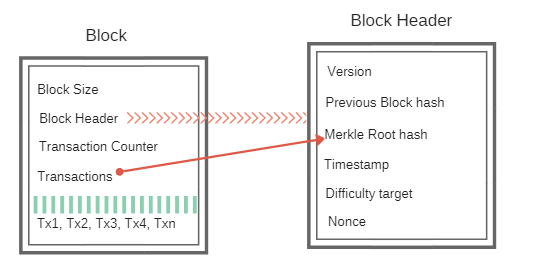
\includegraphics[width=0.755\textwidth]{imgs/block.png}
   \caption{Struttura dei blocchi }
   \end{center}
   \hfill
\end{figure}



\subsection{Identificazione dei blocchi attraverso header e height}
L'identificatore principale di un un blocco \`e il suo \textit{hash} crittografico, una firma digitale, creata applicando per due volte l'algoritmo \textit{SHA256} sull' \textit{header} del blocco stesso, i 32 byte risultanti sono chiamati \textit{block header hash}.\\
L' \textit{hash} identifica univocamente un blocco e pu\`o essere ricalcolato da ogni nodo semplicemente riapplicando lo \textit{SHA256} all' \textit{header} del blocco stesso. \\
Si noti che l' \textit{hash} di un blocco non \`e incluso all' interno della sua struttura dati , invece questo viene calcolato da ogni nodo non appena il blocco \`e propagato nel network.\\
Un secondo modo per identificare un blocco \`e guardando la sua posizione all' interno della \textit{blockchain}, la \textit{block height}.\\
Sebbene un blocco abbia sempre una specifica \textit{height}, il viceversa non \`e sempre vero. Due o pi\`u blocchi possono avere la stessa \textit{height}, quando sono in competizione per la stessa posizione all' interno della \textit{blockchain}, questo scenario \`e chiamato \textit{Blockchain Fork}. Neanche la \textit{block height} fa parte della struttura dati dei blocchi.
\paragraph*{Genesis Block} 
Il primo blocco nella blockchain \`e chiamato \textit{genesis block}, ed \`e stato creato nel 2009. Ogni nodo che entra a far parte del Bitcoin network ha una \textit{blockchain} che al suo interno contiene almeno questo blocco, poich\`e si trova all'interno dell'implementazione \textit{Bitcoin Core}. In questo modo ogni nodo ha un \textit{root} fidato dal quale pu\`o iniziare a costruire la propria catena di blocchi.

\subsection{Collegare i Blocchi nella Blockchain}
I Bitcoin \textit{full node} mantengono una copia locale della \textit{blockchain}, che viene costantemente aggiornata non appena arrivano nuovi blocchi. All' arrivo di un nuovo blocco, il \textit{full node} lo valider\`a e creer\`a un link per collegarlo alla \textit{blockchain} gi\`a esistente, per stabilire questo link il nodo andr\`a a vedere il campo \textit{previous block hash}, cosi da poter stabilire se il padre di questo nuovo blocco corrisponde all' ultimo blocco che lui ha in cima al suo \textit{stack} di blocchi.

\subsection{Merkle Trees}
Ogni blocco della \textit{blockchain} contiene un riepilogo di tutte le transazioni al suo interno tramite il \textit{merkle tree}. Il \textit{merkle tree}, conosciuto anche come \textit{binary hash tree}, \`e una struttura dati utilizzata per  verificare l'integrit\`a di un grande insieme di dati. I \textit{merkle trees} sono quindi alberi binari che contengono \textit{hash} crittografici.\\
Sono usati in Bitcoin per tenere traccia di tutte le transazioni in un blocco, producendo una firma digitale di un intero insieme di transazioni, e fornendo un meccanismo efficiente per verificare se una transazione \`e effettivamente inclusa in un blocco.\\
Il \textit{merkle tree} \`e costruito facendo ricorsivamente \textit{hash} di coppie di nodi fino a che non rimane solamente un nodo, chiamato \textit{root} o \textit{merkle root}. L'algoritmo di \textit{hash} crittografico usato \`e lo \textit{SHA256} applicato due volte.\\
Usando questa struttura, dati \textit{N} elementi all' interno del \textit{merkle tree}, possiamo verificare se uno specifico elemento cui siamo interessati \`e incluso nel \textit{tree} in al pi\`u $2\times\log_2{n}$ calcoli.\\
Il \textit{merkle tree} \`e costruito con un approccio \textit{bottom up}. Nel' esempio in figura \textit{2.8}, si parte da quattro transazioni (A,B,C,D) che formano le foglie dell'albero. Coppie consecutive di nodi sono riassunte nel nodo padre, concatenando i loro due \textit{hash} insieme. Il processo continua finch\`e non rimane solo un nodo in cima all' albero, il \textit{merkle root}. Perci\`o i 32 byte registrati nell' \textit{header} del blocco riassume tutte le transazioni che ne fanno parte.
\begin{figure}[htb]
\begin{center}
   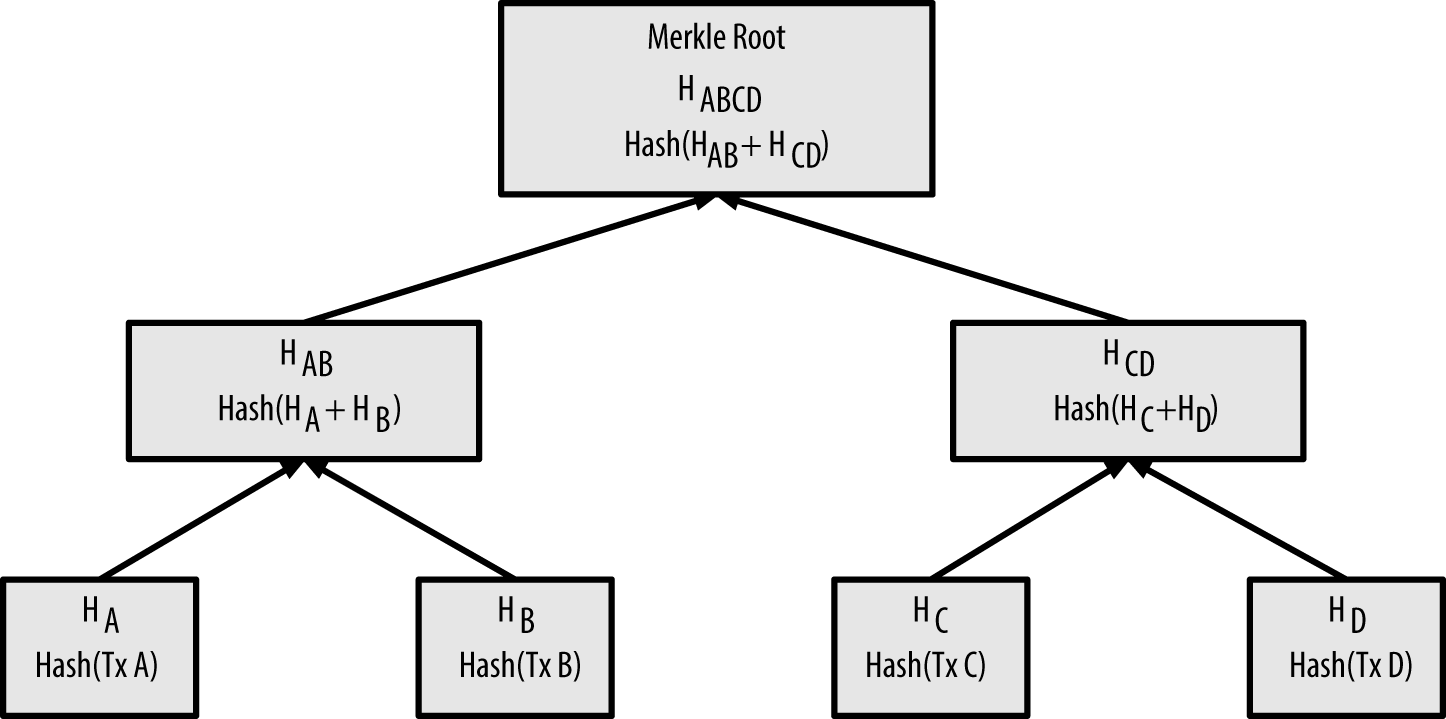
\includegraphics[width=0.755\textwidth]{imgs/merkleTree.png}
   \caption{calcolo dei nodi in un merkle root}
   \end{center}
   \hfill
\end{figure}
Poich\`e il \textit{merkle tree} \`e un albero binario, questo necessita di un numero pari di foglie. Se ci sono un numero dispari di transazioni, l' \textit{hash} dell'ultima transazione viene duplicato per creare un numero pari di foglie, l'albero che cosi viene a crearsi \`e conosciuto con il nome di \textit{balanced tree}.\\
In Bitcoin \`e comune avere migliaia di transazioni incluse in un blocco, quindi possiamo immaginare come le dimensioni dell'albero binario siano molto pi\`u grandi dell'esempio visto precedentemente.\\
Per provare che una transazione \`e davvero inclusa in un blocco, un nodo deve produrre solamente $\log_2{n}$ funzioni di \textit{hash}, costruendo cosi un \textit{authentication path} o \textit{markle path} che connetta quella specifica transazione al root dell'albero.\\
Nella figura seguente producendo un \textit{merkle path} vediamo come si pu\`o provare che la transazione \textit{K} \`e inclusa nel blocco. Il path consiste in quattro funzioni di \textit{hash} che e sono: $H_L,H_{IJ},H_{MNOP},H_{ABCDEFGH}$
\begin{figure}[htb]
\begin{center}
   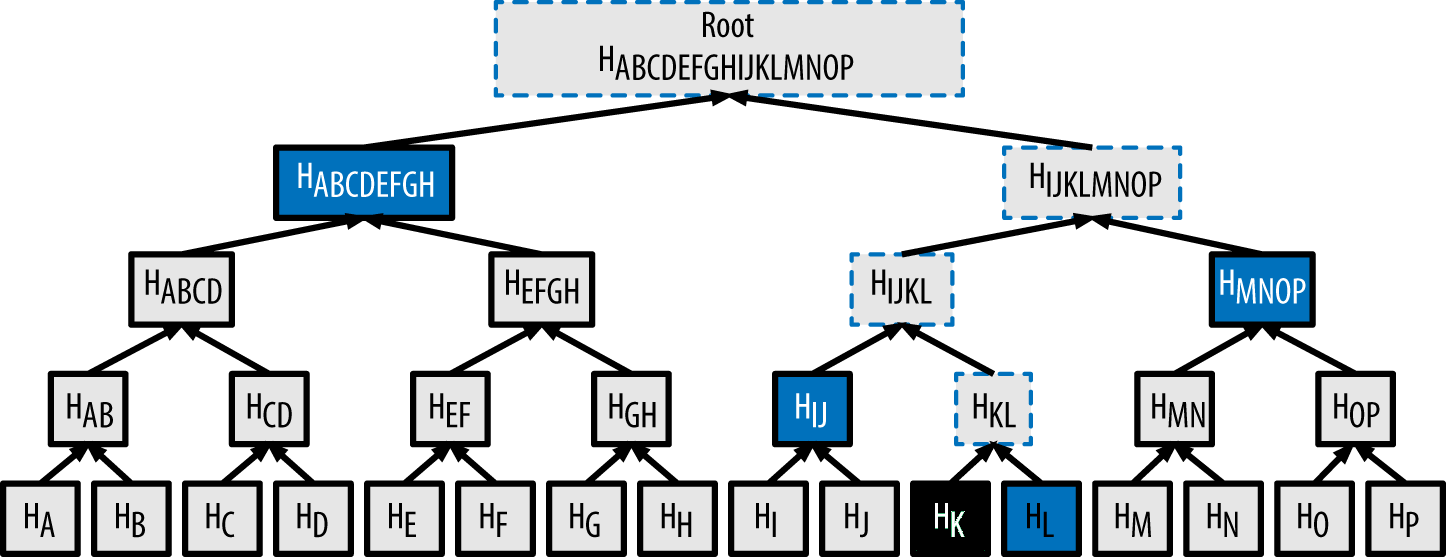
\includegraphics[width=0.755\textwidth]{imgs/merkleProof.png}
   \caption{Merkle path usato per provare l'inclusione dell' elemento K}
   \end{center}
   \hfill
\end{figure}
I nodi \textit{SPV} che non contengono una copia dell' intera \textit{blockchain}, usano i \textit{merkle path} per verificare le transazioni, senza dover fare il download di tutto il blocco.



\section{Mining per il consenso della rete}
\subsection{Introduzione}

L'obbiettivo principale del \textit{mining} non \`e la ricompensa o la generazione di nuovi \textit{coins}, ma il \textit{mining} \`e il meccanismo con il quale le transazioni vengono validate o
eliminate. Il \textit{mining} \`e ci\`o che rende Bitcoin un sistema sicuro e decentralizzato che \`e la base per una moneta digitale basata su rete \textit{P2P}.\\
Il \textit{mining} d\`a sicurezza al sistema Bitcoin e permette di creare moneta \textbf{senza un' autorit\`a centrale}. I \textit{miner} validano le nuove transazioni e le registrano nel \textit{public ledger} (libro mastro). Un nuovo blocco viene "minato" in media ogni 10 minuti. Le transazioni che diventano parte di un blocco e che sono quindi aggiunte alla \textit{blockchain} sono considerate confermate, questo permette al nuovo proprietario dei bitcoin di poter spendere i fondi di quella transazione.\\
I \textit{miner} ricevono due tipi di ricompense: ogni volta che viene minato un blocco vengono creati nuovi \textit{coins} che vengono assegnati al \textit{miner}, e inoltre questi ricevono i \textit{fees} da tutte le transazioni che fanno parte del blocco. Per guadagnare queste ricompense i \textit{miner} devono risolvere un complicato problema matematico basato su un algoritmo di \textit{hash} crittografico. La soluzione a tale problema, chiamato \textit{Proof of Work} \`e inclusa nel nuovo blocco minato, ed \`e prova del lavoro computazionale compiuto dal \textit{miner}.\\
Nuovi bitcoin sono quindi creati grazie al processo di \textit{mining}, in modo del tutto analogo a quando una banca stampa nuove banconote. La quantit\`a di bitcoin che vengono creati all'aggiunta di un nuovo blocco nella \textit{blockchain} diminuisce ogni 4 anni (ogni 210.000 blocchi). Facendo qualche conto si pu\`o notare che la ricompensa di bitcoin sar\`a diminuita esponenzialmente entro il 2140, data in cui non verranno pi\`u generati nuovi bitcoin oltre ai 20.999999998 milioni che saranno gi\`a in circolazione.\\
Abbiamo detto che i \textit{miner} ricevono anche come ricompensa i \textit{fees} da ogni transazione, oggi per\`o la ricompensa in \textit{fees} ricopre solamente il 5\% del guadagno di un \textit{miner}. Ad ogni modo poich\`e generazione di nuovi coins si abbasser\`a esponenzialmente, mentre il numero di transazioni per blocco aumenter\`a , arriver\`a un momento in cui la ricompensa in \textit{fees} sar\`a la parte dominante del guadagno dei  \textit{miner}.




\subsection{Consenso Decentralizzato}
La \textit{blockchain}, come visto nel capitolo precedente, \`e il libro mastro di tutte le transazioni, a cui ogni nodo della rete Bitcoin si affida.\\
Ma come possono tutti fidarsi di una singola \textit{verit\`a}, senza potersi e doversi fidare di nessun' altro all'interno della rete? I metodi di pagamento tradizionali dipendevano sempre da un' figura di autorit\`a centrale, Bitcoin non ha questa figura, ma in qualche modo ogni \textit{full node} ha una copia completa del libro mastro alla quale pu\`o affidarsi. Ogni nodo in qualche modo, attraverso lo scambio di informazioni sul network riesce ad arrivare alla stessa copia del libro mastro.\\
L'invenzione forse pi\`u importante introdotta da Satoshi Nakamoto \`e il meccanismo decentralizzato chiamato \textit{emergent consensus}. Il consenso \`e una caratteristica emergente dell' interazione asincrona di migliaia di nodi indipendenti che seguono delle semplici regole.\\
Il consenso decentralizzato dei Bitcoin emerge dall' interazione di quattro processi che si verificano indipendentemente sui nodi della rete: \
\begin{itemize}
\item Verifica indipendente di ogni transazione da parte di ogni \textit{full node}:\\
prima di propagare una transazione all'interno del network i \textit{full node} verificano che la transazione sia valida, in caso negativo questa sar\`a gi\`a scartata dal primo nodo.
\item Aggregazione indipendente di quelle transazioni nei nuovi blocchi fatta dai nodi \textit{miner}, attraverso la computazione della \textit{Proof of Work}.
\item Verifica indipendente dei nuovi blocchi , da ogni nodo e assemblamento in un catena.
\item Selezione indipendente da ogni nodo, della catena con pi\`u lunga.
\end{itemize}



\subsection{Aggregare Transazioni nei Blocchi}
Dopo aver validato le transazioni, un nodo Bitcoin le aggiunge nella \textit{memory/transaction pool}, dove queste attendono di essere incluse in un bloccco.\\
Descriviamo con un esempio ora il procedimento che compie un nodo \textit{miner} all'interno della rete.\\
Il nodo \textit{miner} di Gianni mantiene una copia locale della \textit{blockchain}. Allo stesso tempo Alice sta comprando una tazza di caff\`e, in questo momento la \textit{blockchain} di Gianni contiene 277,324 blocchi. Il nodo di Gianni rimane in ascolto per ricevere sempre nuove transazioni, prova a minare un nuovo blocco e inoltre controlla se qualche blocco \`e stato aggiunto da qualche altro \textit{miner} alla \textit{blockchain}.\\
Mentre il nodo di Gianni sta minando sfortunatamente viene annunciato il blocco 277,315 , cosi inizia subito la competizione per il blocco 277,316.\\
Durante i 10 minuti precedenti, mentre Gianni cercava di minare il blocco 277,315, stava allo stesso tempo collezionando transazioni da includere nel blocco. Adesso dovr\`a controllare che tra le transazioni che ha collezionato non ce ne sia qualcuna inclusa nel blocco 277,315, in tal caso dovr\`a eliminarla dalla \textit{transaction pool}.\\
Gianni costruisce immediatamente un blocco vuoto, candidato per la posizione 277,316, che viene appunto chiamato \textit{candidate block}, poich\`e il \textit{miner} ancora non ha trovato una soluzione all'algoritmo di \textit{Proof-of-Work}.

\subsection{La Transazione Coinbase}
La prima transazione in ogni blocco \`e speciale, viene chiamata \textit{coinbase transaction}. Questa transazione viene costruita dal nodo i Gianni come ricompensa degli sforzi fatti.\\
A differenza della transazioni comuni, la \textit{coinbase} non consuma \textit{UTXO} per i suoi input, invece ha solamente un input chiamato \textit{coinbase}.


\subsection{Minare il Blocco}
Adesso che il nodo di Gianni \`e stato costruito, \`e tempo di minare il blocco, trovando una soluzione al \textit{Proof of Work} che renda il blocco valido.\\
In termini semplici, minare \`e il processo in cui vengono eseguite tante funzioni di \textit{hash} ripetutamente, cambiando un solo parametro, fin tanto che il risultato dell'\textit{hash} non combaci con uno specifico target. Il risultato della funzione di \textit{hash} non pu\`o essere predeterminato, questa caratteristica fa in modo che l'unica maniera di produrre degli \textit{hash} che combacino con uno specifico target sia solamente provando e riprovando in modo del tutto casuale, modificando l'input.


\subsection{Algoritmo Proof-of-Work}
Un algoritmo di \textit{hash} prende in input un dato di lunghezza arbitrariamente lunga e produce un risultato di lunghezza fissa, la firma digitale dell'input. Per ogni specifico input, il risultato della funzione di \textit{hash} sar\`a sempre lo stesso. La caratteristica principale di un algoritmo di \textit{hash} crittografico \`e che \`e computazionalmente impossibile trovare due differenti input che producano la stessa firma (situazione nota come \textit{collisione}).\\
Con l'algoritmo di \textit{hash} usato in Bitcoin, \textit{SHA256}, l'output ha una lunghezza fissa di 256 bit. Vediamo degli esempi in cui ad una particolare stringa viene aggiunto un numero (\textit{nonce}) che cambia continuamente e alla quale applichiamo l'\textit{l'hash} crittografico:\\
Io sono Marcello Politi0 := a80a81401765c8eddee25df36728d732...\\
Io sono Marcello Politi1 := f7bc9a6304a4647bb41241a677b5345f...\\
Io sono Marcello Politi2 := ea758a8134b115298a1583ffb80ae629...\\
Io sono Marcello Politi3 := bfa9779618ff072c903d773de30c99bd...\\
Io sono Marcello Politi4 := bce8564de9a83c18c31944a66bde992f...\\
Io sono Marcello Politi5 := eb362c3cf3479be0a97a20163589038e...\\
Io sono Marcello Politi6 := 4a2fd48e3be420d0d28e202360cfbaba...\\
Io sono Marcello Politi7 := 790b5a1349a5f2b909bf74d0d166b17a...\\
Io sono Marcello Politi8 := 702c45e5b15aa54b625d68dd947f1597...\\
Io sono Marcello Politi9 := 7007cf7dd40f5e933cd89fff5b791ff0...\\
Io sono Marcello Politi10 := c2f38c81992f4614206a21537bd634a...\\
Io sono Marcello Politi11 := 7045da6ed8a914690f087690e1e8d66...\\
Io sono Marcello Politi12 := 60f01db30c1a0d4cbce2b4b22e88b9b...\\
Io sono Marcello Politi13 := 0ebc56d59a34f5082aaef3d66b37a66...\\
Si pu\`o notare che cambiando soltanto il \textit{nonce} finale, l'\textit{hash} della stringa cambia totalmente.\\
Per complicare un p\`o il tutto, fissiamo un target: troviamo quindi una stringa che produca un \textit{hash} esadecimale che inizi con la cifra 0. Fortunatamente non \`e difficile, se vediamo il tredicesimo tentativo rispetta i nostri criteri. In termini di probabilit\`a, se gli output della funzione di \textit{hash} sono equamente distribuiti, ci aspettiamo di trovare uno 0 in prima posizione una volta ogni 16 tentativi in media.\\
Notiamo anche che l'obbiettivo da noi posto equivale a trovare un \textit{hash} inferiore a:\\
0x1000000000000000000000000000000000000000000000000000000000000000\\
che \`e appunto il nostro \textit{target}. Se abbassassimo il target il nostro obbiettivo diventerebbe sempre pi\`u difficile.\\
Per capire meglio facciamo una semplice analogia. Immaginiamo un gioco in cui i giocatori tirano due dadi, e la somma di questi deve essere inferiore ad un certo target. Inizialmente il target \`e 12, quindi a meno che non si lanci un doppio 6, vinciamo sicuramente, quindi sembra in questo caso che il gioco sia molto semplice. Andando avanti per un paio di turni il target si abbassa a 5. Adesso notiamo che pi\`u del doppio dei lanci che possiamo fare risulter\`a fuori target, il gioco \`e diventato molto pi\`u difficile da vincere. Nel caso i target sia 2 (il minimo possibile) abbiamo solo un lancio che ci far\`a vincere, e in questo caso ci aspettiamo che di tirare un doppio 1 una volta ogni 36 lanci. In questo modo possiamo fare una stima dei lanci che abbiamo bisogno di fare per vincere, e questo ci da una prova che abbiamo fatto diversi tentativi prima di vincere, lo stesso vale quindi per i \textit{miner}, il fatto che trovino un \textit{hash} che rispetti il target \`e un \textit{proof} (prova) \textit{of work} (del lavoro fatto).\\
Nell' esempio mostrato precedentemente il \textit{nonce} vincente era il numero 13, e questo risultato pu\`o essere confermato da qualunque nodo indipendentemente. Tutti possono aggiungere il suffisso "13" alla frase "Io sono Marcello Politi" ed eseguirne l'\textit{hash} per vedere che quello che ne viene fuori sia un numero minore del target. Conoscendo il target ognuno pu\`o fare una stima della difficolt\`a di risolvere la \textit{Proof of Work} e conoscere quindi quanto lavoro ci vuole per trovare il \textit{nonce}.\\
Abbiamo gi\`a visto come un \textit{miner} costruisce un \textit{candidate block} pieno di transazioni. Successivamente il \textit{miner} calcola l' \textit{hash} dell'\textit{header} del blocco e verifica che sia pi\`u piccolo del target, se non lo \`e il \textit{miner} modificher\`a il \textit{nonce} e prover\`a nuovamente.


